% !TEX TS-program = xelatex
% !TEX encoding = UTF-8 Unicode
\documentclass[11pt,a4paper]{article}
\usepackage{amsmath,amssymb}
\usepackage{empheq}
\usepackage[semibold]{ebgaramond}
\usepackage[cmintegrals,cmbraces]{newtxmath}
\usepackage{ebgaramond-maths}
\usepackage{bm}
\usepackage[OMLmathrm, OMLmathsfit, rmdefault=mdugm]{isomath}
\usepackage{tocbibind}

\makeatletter
  \DeclareSymbolFont{ntxletters}{OML}{ntxmi}{m}{it}
  \SetSymbolFont{ntxletters}{bold}{OML}{ntxmi}{b}{it}
  \re@DeclareMathSymbol{\leftharpoonup}{\mathrel}{ntxletters}{"28}
  \re@DeclareMathSymbol{\leftharpoondown}{\mathrel}{ntxletters}{"29}
  \re@DeclareMathSymbol{\rightharpoonup}{\mathrel}{ntxletters}{"2A}
  \re@DeclareMathSymbol{\rightharpoondown}{\mathrel}{ntxletters}{"2B}
  \re@DeclareMathSymbol{\triangleleft}{\mathbin}{ntxletters}{"2F}
  \re@DeclareMathSymbol{\triangleright}{\mathbin}{ntxletters}{"2E}
  \re@DeclareMathSymbol{\partial}{\mathord}{ntxletters}{"40}
  \re@DeclareMathSymbol{\flat}{\mathord}{ntxletters}{"5B}
  \re@DeclareMathSymbol{\natural}{\mathord}{ntxletters}{"5C}
  \re@DeclareMathSymbol{\star}{\mathbin}{ntxletters}{"3F}
  \re@DeclareMathSymbol{\smile}{\mathrel}{ntxletters}{"5E}
  \re@DeclareMathSymbol{\frown}{\mathrel}{ntxletters}{"5F}
  \re@DeclareMathSymbol{\sharp}{\mathord}{ntxletters}{"5D}
  \re@DeclareMathAccent{\vec}{\mathord}{ntxletters}{"7E}
\makeatother

\usepackage{array}
\usepackage{enumitem}
% to produce a comma between multiple footnotes / https://tex.stackexchange.com/questions/40072/incompatibility-between-footmisc-option-multiple-and-hyperref/62091#62091
\let\oldFootnote\footnote
\newcommand\nextToken\relax
\renewcommand\footnote[1]{%
    \oldFootnote{#1}\futurelet\nextToken\isFootnote}
\newcommand\isFootnote{%
    \ifx\footnote\nextToken\textsuperscript{,}\fi}

\defaultfontfeatures{Ligatures=TeX} % makes this a feature for all selected fonts
\usepackage{esint}
\usepackage{polyglossia}
\setmainlanguage{english}
\usepackage[text={18cm,26cm},centering]{geometry} % 
\usepackage{natbib}
\usepackage{graphicx}
\graphicspath{{./pics/}}
\usepackage{wrapfig}
\usepackage{mdframed}
\usepackage{lipsum}
\usepackage[usenames,dvipsnames,svgnames,table]{xcolor}
\usepackage{hyperref}
\usepackage{url}
\usepackage[export]{adjustbox}

\hypersetup{
  colorlinks,
  citecolor=bleuSU,
  linkcolor=bleuSU
}
\definecolor{bleuSU}{RGB}{26,39,101}

\usepackage[normalem]{ulem}
\makeatletter
\renewcommand*{\uuline}{%
  \bgroup
  \UL@setULdepth
  \markoverwith{%
    \lower\ULdepth\hbox{%
      \kern-.03em%
      \vtop{%
        \hrule width.2em%
        \kern 0.6pt % distance between the two underlines
        \hrule
      }%
      \kern-.03em%
    }%
  }%
  \ULon
}
\makeatother
\setlength{\ULdepth}{-2pt}  % distance from double underline to letter

\usepackage{environ}
\newtoggle{corrige}

\NewEnviron{answer}{%
  \iftoggle{corrige}
    {\begin{mdframed}\textbf{Answer: } \BODY\end{mdframed}}
    {}%
  }

\newcommand{\delS}{\delta S}
\newcommand{\delA}{\delta A}
\newcommand{\delh}{\delta h}
\newcommand{\delt}{\delta t}
\newcommand{\delz}{\delta z}
\newcommand{\delbx}{\delta \matrixsym x}
\newcommand{\lp}{\left(}
\newcommand{\rp}{\right)}
\newcommand{\itA}{\textit A}
\newcommand{\itB}{\textit B}
\newcommand{\dAB}{\mathcal D_{AB}}
\newcommand{\bA}{\matrixsym A}
\newcommand{\bff}{\matrixsym{f}}
\newcommand{\bF}{\matrixsym{F}}
\newcommand{\bj}{\matrixsym{j}}
\newcommand{\bJ}{\matrixsym J}
\newcommand{\bn}{\matrixsym{n}}
\newcommand{\bN}{\matrixsym N}
\newcommand{\bP}{\matrixsym{P}}
\newcommand{\br}{\matrixsym r}
\newcommand{\bt}{\matrixsym t}
\newcommand{\be}{\matrixsym e}
\newcommand{\bu}{\matrixsym u}
\newcommand{\bv}{\matrixsym v}
\newcommand{\bw}{\matrixsym w}
\newcommand{\bx}{\matrixsym x}
\newcommand{\pd}[2]{\frac{\partial #1}{\partial #2}}
\newcommand{\dx}[1]{\frac{\partial  #1}{\partial x}}
\newcommand{\dy}[1]{\frac{\partial  #1}{\partial y}}
\newcommand{\dz}[1]{\frac{\partial  #1}{\partial z}}
\newcommand{\dr}[1]{\frac{\partial  #1}{\partial r}}
\newcommand{\drs}[1]{\frac{\partial^\star  #1}{\partial r^\star}}
\newcommand{\dt}[1]{\frac{\partial  #1}{\partial t}}
\newcommand{\D}[2]{\frac{D #1}{D #2}}
\newcommand{\dd}[2]{\frac{\mathrm d #1}{\mathrm d #2}}
\newcommand{\dA}{\mathrm dA}
\newcommand{\dV}{\mathrm dV}
\newcommand{\dS}{\mathrm dS}
\newcommand{\prg}[1]{\paragraph{$\rhd$ #1}}
\newcommand{\alphaijkl}{\alpha_{ijkl}}
\newcommand{\Aijkl}{A_{ijkl}}
\newcommand{\delij}{\delta_{ij}}
\newcommand{\sigij}{\sigma_{ij}}
\newcommand{\sigji}{\sigma_{ji}}
\newcommand{\sigxy}{\sigma_{xy}}
\newcommand{\matL}{\mathcal L}
\newcommand{\matO}{\mathcal O}
\newcommand{\matS}{\mathcal S}
\newcommand{\kij}{k_{ij}}
\newcommand{\tensor}[1]{\smash{\uuline{#1}{}}}
\setlength{\parindent}{0pt} % remove indent
  
\begin{document}
\setlength{\unitlength}{1cm}
\noindent
\parbox{\textwidth}{
\textsc{
Sorbonne Université  
\hfill
Year 2021-2022
}
}
\parbox{\textwidth}{
\textsc{
Faculté des Sciences
\hfill
Physics of Fluids \& Nonlinear Physics
}
}

\begin{center}
\Large
\textbf{Hydrodynamics} \\ 
\textsl{Tutorial 1: fluid motion} \\[1ex]
\end{center}

%\vspace{5mm}
\section{Dimensional analysis}
\toggletrue{corrige}

\paragraph{$\rhd$ Imbibition.}  
\begin{figure}[ht]
    \centering
    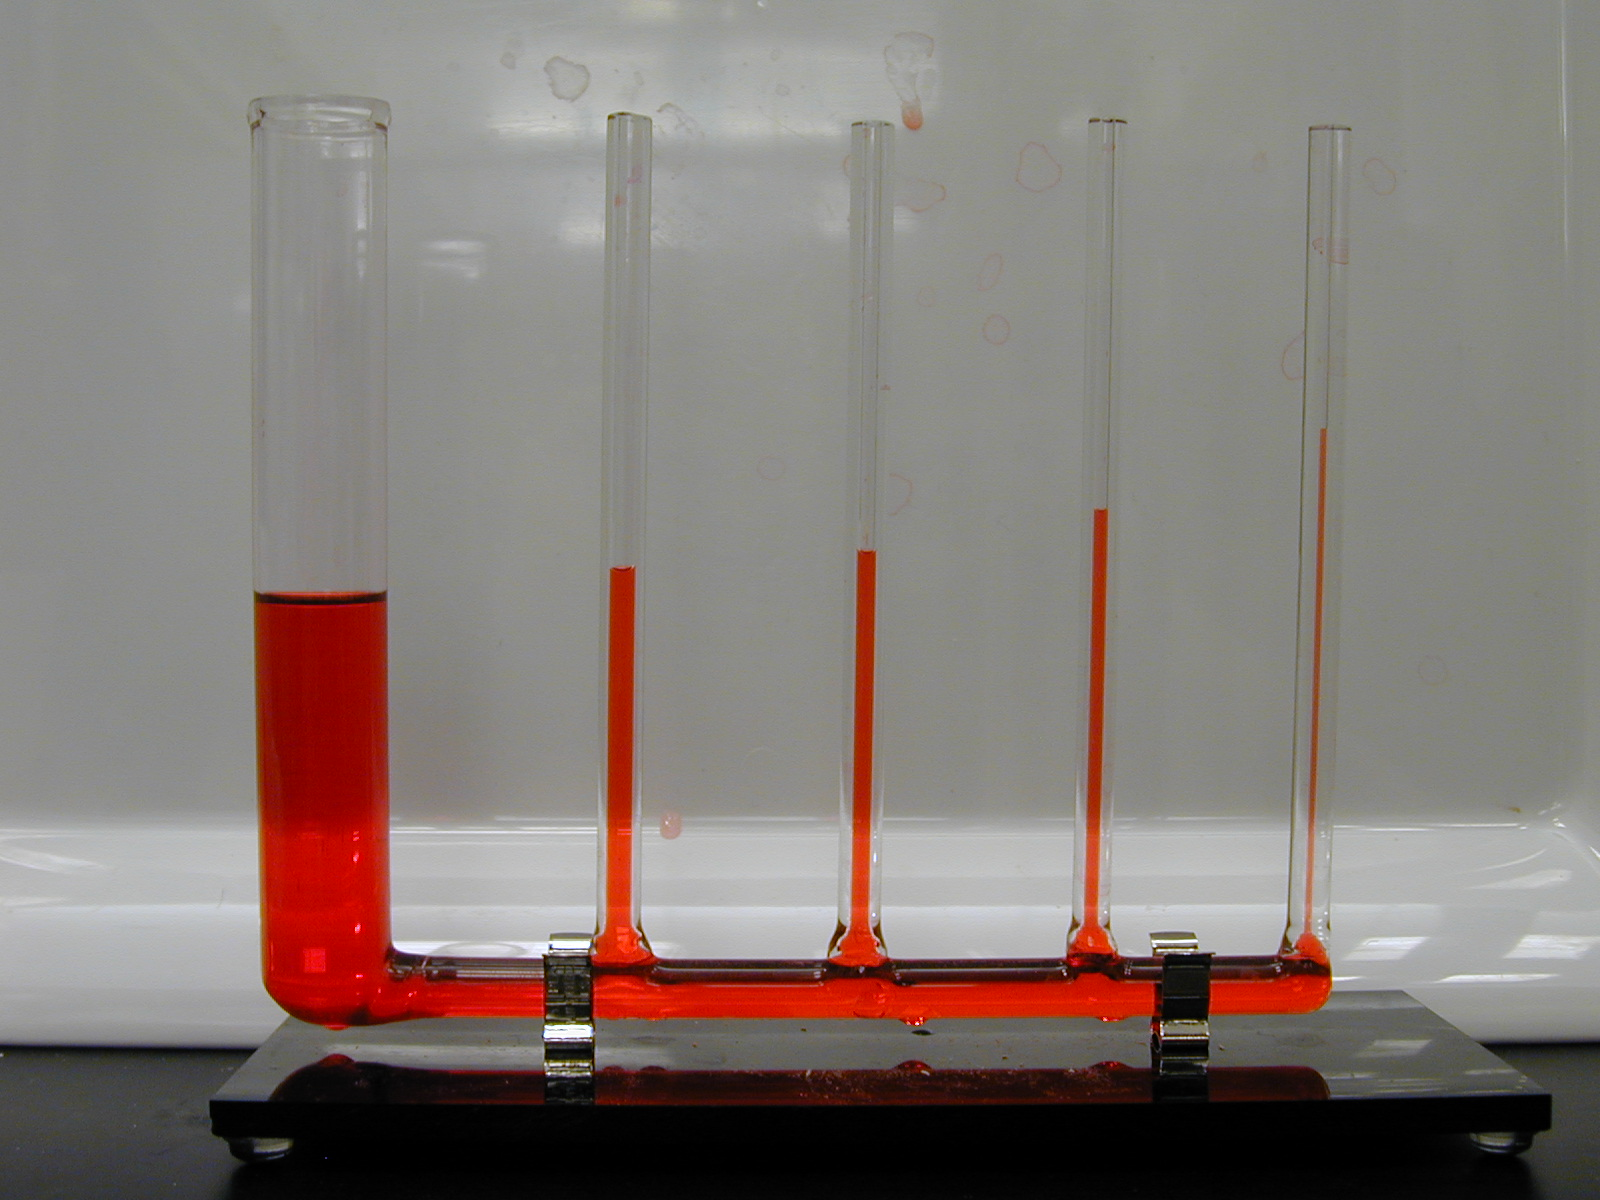
\includegraphics[height=5cm,valign=m]{capillaryrise.JPG}
    \hspace{1cm}
    \includegraphics[valign=m,page=2]{lucas.pdf}
    \caption{\textbf{Maximal ascension.} Left: the maximal height for capillary ascension depends on tube radius $R$. Right: maximal height $h$ observed for the capillary rise of ethanol in tubes of different radii $R$ (data from the authors).}
    \label{fig:jurin}
\end{figure}
A narrow capillary tube is brought into contact with a wetting liquid. The liquid spontaneously rises in the tube up to a height $h$ (figure~\ref{fig:jurin}). This height depends a priori on the \textit{surface tension} $\gamma$ ($[\gamma] = \mathsf{MT}^{-2}$), gravity $g$, density $\rho$ and on the tube radius $R$ :
\begin{equation}
h = f(\gamma, \rho, g, R)
\end{equation}
\begin{enumerate}
\item Using the characteristic scales $\rho$, $g$ and $R$, show that the previous functional relation can be rewritten as:
\begin{equation}
\mathrm \pi = \mathcal F(\mathrm \pi_1),
\end{equation}
where $\mathrm \pi$ corresponds to the nondimensional height (the observable), and $\mathrm\pi_1$ to the non-dimensional surface tension. Write the expression for $\mathrm\pi$ and $\mathrm\pi_1$ (that we will take proportional to $h$ and $\gamma$ respectively).
\begin{answer}
\begin{equation*}
\pi = \frac{h}{R} \quad \text{ and } \quad \pi_1 = \frac{\gamma}{\rho g R^2}
\end{equation*}
\end{answer}

\item Experiments and physical analysis show that $\mathcal F(x) = 2x$. What is the scaling law of $h$ with respect to $R$ ? Is it compatible with the experimental results reported~\ref{fig:jurin} ?
\begin{answer}
We have $h = \frac{2\gamma}{\rho g R}$ therefore $h \propto \frac{1}{R}$, compatible with the experimental results.
\end{answer}
\end{enumerate}

\paragraph{$\rhd$ Molecular diffusion.} A drop of dye is delicately deposited in a liquid. Due to constant molecular motion and collisions, the area expands by \textit{diffusion} -- a process whose efficiency is characterised with the diffusion coefficient $D$ (of dimension $[D] = \mathsf{L^2T^{-1}}$). 
\begin{enumerate}[resume]
\item Using dimensional analysis show that the dye drop spreads following a square root law at long times $R(t) \propto t^{1/2}$.
\begin{answer}
$h = a \sqrt{Dt}$
\end{answer}
\end{enumerate}
\paragraph{$\rhd$ Turbulent diffusion.} \textit{(from \citet{Eggers2015})}. We consider again the previous experiment but now the liquid is vigorously stirred, so as as to create turbulent motions stirring and mixing the dye. This process is a priori much more efficient than simple molecular diffusion, so that we neglect the latter in the following. The stirring intensity is characterised with $\varepsilon$, the energy quantity per unit time and mass in the liquid. 
\begin{enumerate}[resume]
\item what is the dimension of $\varepsilon$ ?
\begin{answer}
$[\varepsilon] = \mathsf{L}^2\mathsf{T}^{-3}$
\end{answer}

\item Show that the drop area now grows according to
\begin{equation}
R(t) = A \lp \varepsilon t^3\rp^{1/2},
\end{equation}
where $A$ is a dimensionless universal constant. This result is the signature of a process much more efficient than molecular diffusion, and known as \textit{Richardson's law} \citep{Richardson1926,Eggers2015}.
\end{enumerate}

\section{Tumbling cards}

\begin{figure}[ht]
    \centering
    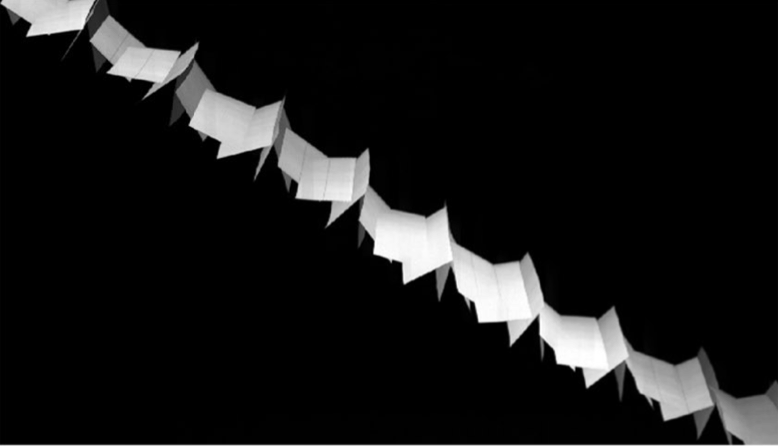
\includegraphics[height=4cm,valign=t]{ristroph.png}
    \hspace{1cm}
    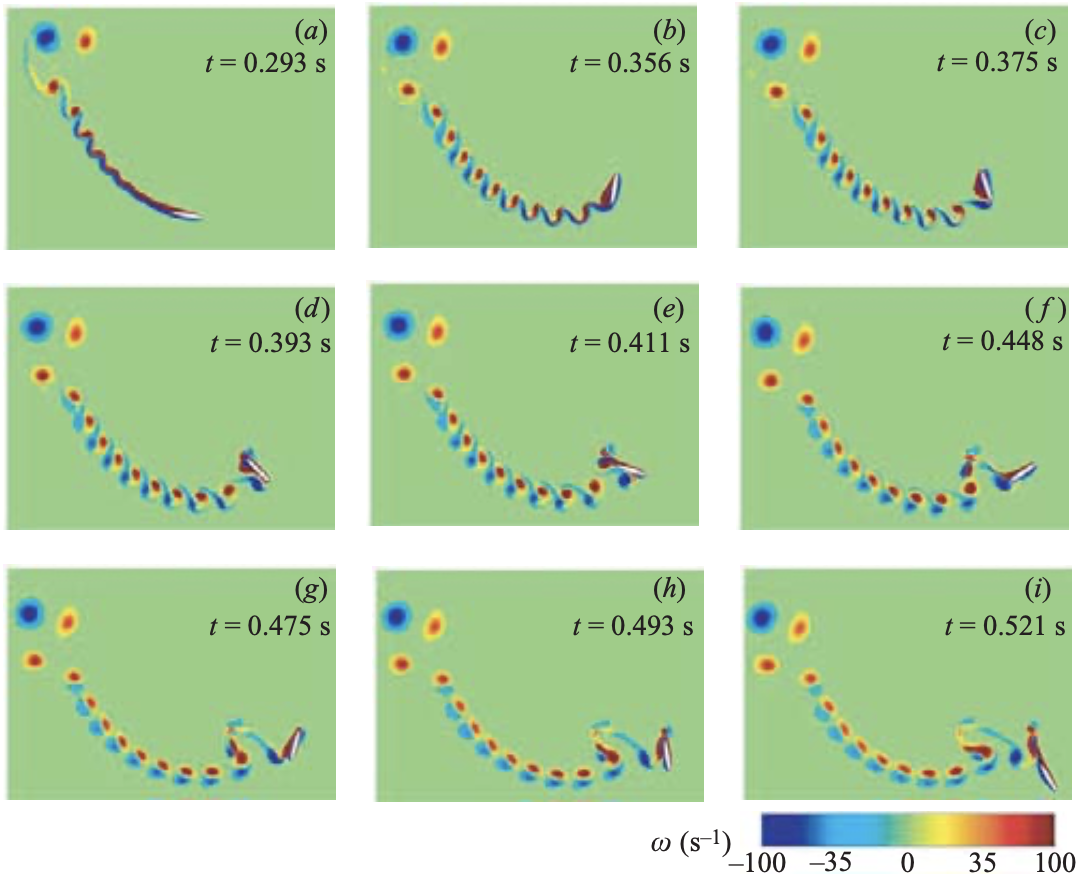
\includegraphics[height=5cm,valign=t]{andersen.png}
    \caption{\textbf{Tumbling cards.} Left: chronophotograph of a falling and tumbling card. Right: numerical simulations of the process reveal an intricate vortex wake associated with boundary layer detachment.}
    \label{fig:tumbling}
\end{figure}
Freely falling cards or metro tickets naturally tumble when falling. The observable frequency of tumbling is the result from an intricate process coupling the card flight with a complex vortex wake, see Fig.~\ref{fig:tumbling}. Here we will see how experiments and dimensional analysis can help us in obtaining quantitative predictions about the frequency.
\begin{enumerate}
\item By cutting out cards from a piece of paper, observe the tumbling phenomenon.
\item Identify the key parameters influencing the frequency $\Omega$ \textit{a priori}. We will denote the length of the card $l$, its width $w$ and thickness $t$. The density of the card will be denoted $\rho_c$ and that of air $\rho_a$. Are there other relevant parameters?
\item From the experiments, observe qualitatively the independence of $\Omega$ with $l$.
\item Experiments further reveal that the tumbling is insensitive to the nondimensional air viscosity (Reynolds or Archimedes number). For fixed density ratios, show the nondimensional frequency ultimately depend on a single nondimensional parameter.
\item Using the dataset given as supplementary material, find the scaling law linking these two parameters. Conclude on the tumbling frequency scaling law. 
\item In order to shed further light on this scaling, further experiments reveal that the descent velocity $V$ follow the scaling $V \sim \Omega w$. Using this result, show that an order of magnitude balance between weight and drag allows to recover the tumbling frequency scaling.
\end{enumerate}

\section{Starting plane shear flow}
\begin{figure}[h]
\begin{center}
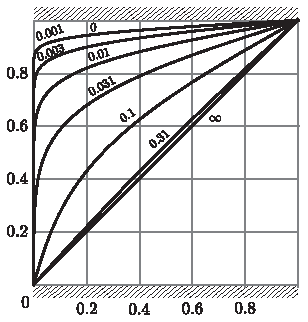
\includegraphics{transient_couette.pdf}
\end{center}
\caption{\textbf{Transient of a Couette flow}. Several successive velocity profiles are shown here as a function of the nondimensional time $\bar t = \nu t / h^2$.}
\end{figure}

\noindent We are interested here in the setting up of a fluid flowing in between two parallel plates of infinite extension when one of them is suddenly set into motion \citep{Batchelor1967,Ockendon1995}. The plates are separated with a distance~$h$. At $t=0$ the upper plate is abruptly set into motion at velocity $\matrixsym U = (U,0,0)$. The fluid, at rest until that moment, starts progressively to move due to momentum diffusion until it reaches the Couette steady-state. Note also that there is no imposed pressure gradient and that momentum diffusion is the only cause for fluid motion. The dynamic viscosity of the fluid is noted~$\mu$, the kinematic viscosity $\nu$ and we neglect the action of gravity. We will consider an translation-invariant evolution along the two directions parallel to the plates (this amounts to consider a \textbf{parallel} flow) and we will also suppose that the flow is \textbf{incompressible}\footnote{Over very short times of the order $h/c$ with $c$ the sound celerity in the fluid, this hypothesis can be invalidated. But we can put figures to get an idea by taking e.g. water as a working fluid ($c\simeq 1500 \text{m}\cdot\text{s}^{-1}$) and $h = 1 \text{cm}$ as the distance between the plates. The acoustic timescale. is then of the order of 7 $\mu$s to be compared with the diffusive timescale exceeding a minute (7 orders of magnitude apart!). Moreover it is quite possible that in the experimental setup the starting of the plate cannot be considered impulsive over the acoustic timescale.}.
\begin{enumerate}
    \item Propose an estimation of the order of magnitude of the viscous shear stress exerted on one of the plate in the steady limit, along with an estimation of the typical transient timescale.
\begin{answer}
The viscous shear stress $\tau$ corresponds to the product between viscosity and the wall shear, that we can estimate here with $U/h$.
 We therefore get:
 $$
 \tau \sim \mu \frac{U}{h}.
 $$
The typical transient timescale is a \textbf{diffusive} timescale (vertical diffusion of horizontal momentum) and is $h^2/\nu$.
\end{answer}
    \item Write down the equations expressing mass and momentum conservation (using scalar projections), along with the boundary conditions and the initial condition of the problem. Beware of neglecting the unsteady terms.
    \begin{answer}
    The 2D equations of motion and mass conservation read, for this incompressible evolution:
\begin{subequations}
\begin{empheq}[left=\empheqlbrace]{alignat=1}
\rho\left(\dt{u}+u\dx{u}+v\dy{u}\right) &= -\pd{p}{x} + \mu \left(\frac{\partial^2u}{\partial x^2} + \frac{\partial^2u}{\partial y^2} \right)\notag\\
\rho\left(\dt{v}+u\dx{v}+v\dy{v}\right) &= -\pd{p}{y} + \mu \left(\frac{\partial^2v}{\partial x^2} + \frac{\partial^2v}{\partial y^2} \right)\notag\\
\pd{u}{x}+\pd{v}{y}&=0\notag
\end{empheq}
\end{subequations}
These equations are associated to impermeability and no-slip boundary conditions:
$$
u(x,0,t) = 0 ; \quad u(x,h,t) = U ; \quad  v(x,0,t) = 0 ; \quad  v(x,h,t) = 0.
$$
Finally at initial time, the fluid is at rest:
$$
u(x,y,0) = v(x,y,0) = 0.
$$
Enforcing $x$-translation invariance and no longitudinal pressure gradient allows to simplify the equations:
\begin{subequations}
\begin{empheq}[left=\empheqlbrace]{alignat=1}
\rho\left(\dt{u}+v\dy{u}\right) &= \mu  \frac{\partial^2u}{\partial y^2} \notag\\
\rho\left(\dt{v}+v\dy{v}\right) &= -\pd{p}{y} + \mu \frac{\partial^2v}{\partial y^2} \notag\\
\pd{v}{y}&=0\notag
\end{empheq}
\end{subequations}
The last equation, combined to the boundary conditions on the vertical velocity, shows that $v=0$ everywhere in the fluid. It follows that pressure is constant throughout the fluid.

Finally the equations can be simplified to:
$$
\dt{u} = \nu  \frac{\partial^2u}{\partial y^2} \notag
$$
associated to
$$
u(0,t) = 0 ; \quad u(h,t) = U ; \quad  u(y,0) = 0.
$$
\end{answer}
     \item Nondimensionalise the equations using the natural scales of the problem by setting $y = h \bar y, u = U \bar u$ and $t = h^2 \bar t / \nu$. 
    \begin{answer}
    We get :
    $$
    \pd{\bar u}{\bar t} = \frac{\partial^2 \bar u}{\partial \bar y^2},
    $$
    associated to 
    \begin{empheq}[left=\empheqlbrace]{alignat=2}
&\text{bottom plate no-slip condition} :\qquad &  \bar u(0,\bar t) = 0,\nonumber \\
&\text{upper plate no-slip condition} :\qquad & \bar u(1,\bar t) = 1,\nonumber\\
&\text{initial condition} :\qquad & \bar u(\bar y,0) = 0.\nonumber
\end{empheq}
    \end{answer}
    \item In the steady limit, determine the flow profile $\bar u_\text{couette}(\bar y)$ along with its gradient, and deduce the dimensioned value of the wall shear stress both at the bottom and at the top plate. 
\begin{answer}
$\bar u_\text{couette}(\bar y) = \bar y$ so $\dd{}{\bar y}\bar u_\text{couette}(\bar y) = 1$ hence $\tau = \mu \frac{U}{h} \dd{}{\bar y}\bar u_\text{couette}(\bar y) = \mu \frac{U}{h}$.
\end{answer}
\end{enumerate}

\noindent We now seek to describe the onset of this flow with a solution of the form:
\begin{equation}
\bar u(\bar y,\bar t) = \bar u_\text{couette}(\bar y) + \bar u_\text{unst}(\bar y,\bar t)
\label{eq:profile}
\end{equation}
\begin{enumerate}[resume]
    \item Injecting the profile~(\ref{eq:profile}) in the equations for motion, obtain a new set of equations and boundary conditions for $\bar u_\text{unst}(\bar y,\bar t)$. What is the initial condition for  $\bar u_\text{unst}(\bar y,0)$ ? 
    \begin{answer}
    Same equation (linearity). Homogeneous BC for $\bar u_\text{unst}$ and $\bar u_\text{unst}(\bar y,0) = -\bar y$.
    \end{answer}
    \item We look for a solution by using the variable separation technique, i.e. we pose $\bar u_\text{unst}(\bar y,\bar t) = f(\bar y)g(\bar t)$. Obtain the equations governing $f(\bar y)$ and $g(\bar t)$ along with the general form of the solutions.
\begin{answer}
We have:
$$
\frac{g'}{g} = \frac{f''}{f} = \pm K^2
$$
The sign of the constant sets the time behaviour of the solution ($+K^2$ implies an exponentially growing solution, $-K^2$ an exponentially decaying, and 0 an algebraically growing or decaying solution -- or a constant). We seek to describe a relaxation process so the choice $-K^2$ is the only physically sound. The general solution has therefore the form:
$$
u(\bar y,\bar t) = \int_k \left(A(k) \cos(k \bar y) + B(k) \sin(k \bar y)\right) e^{-k^2 \bar t} \, \mathrm dk.
$$
\end{answer}
    \item Show that the application of the boundary conditions imposes a quantisation condition on the solutions. Deduce the form of the velocity profile as a Fourier series whose coefficients are yet to be determined.
\begin{answer}
The bottom boundary condition implies $A(k) = 0$. The top boundary condition cannot be fulfilled \textit{unless} $\sin(k) = 0$, which is possible for the discrete set of wavenumbers $k = n\pi$, $n \in \mathbb{N}$ (there is no need to consider negative values for $k$ as they describe the same functions as their positive opposite. Further $k=0$ represents the null function and can be disregarded). Finally, the general form of the solution satisfying all the boundary conditions is:
$$
u(\bar y, \bar t) = \sum_{n=1}^\infty a_n \sin(n \pi \bar y) e^{-n^2 \pi^2 \bar t}.
$$
\end{answer}
    \item Demonstrate the orthogonality relation:
    $$
     \int_0^1 \sin(n \pi x) \sin(m \pi x) \, \mathrm dx = \begin{cases*} 0 & if  $n \neq m$ \\ \frac{1}{2} & if $n = m$ \end{cases*}
    $$
\begin{answer}
The idea is here to linearise this expression with single cosines, and then perform the integration. We have:
$$
\sin(n \pi x)\sin(m \pi x) = \frac{1}{2}\left(\cos((n-m)\pi x)-\cos((n+m)\pi x)\right).
$$
We note that 
$$
\int_0^1 \cos(j \pi x) \, \mathrm dx = \begin{cases*} \frac{1}{j\pi}\left[\sin(j\pi x)\right]_0^1=0 & if  $j \neq 0$ \\ 1 & if $j = 0$ \end{cases*}
$$
Hence the result.
\end{answer}
    \item Exploit the orthogonality relation so as to determine the flow transient, then show that the dimensioned expression for the velocity field is
    \begin{equation}
    u(y,t) = \frac{U y}{h} + \sum_{n=0}^\infty \frac{2U}{n\mathrm\pi} \lp-1\rp^n \sin\lp\frac{n\mathrm\pi y}{h}\rp e^{-\frac{n^2 \mathrm\pi^2}{h^2}\nu t}
    \end{equation}
\begin{answer}
The initial condition is:
$$
\bar u_\text{unst}(\bar y,0) = -\bar y = \sum_{m=1}^\infty a_m \sin(m \pi \bar y)
$$
Multiplying this equation on both sides by $\sin(n \pi \bar y)$ and integrating over the fluid gap, we have:
$$
-\int_{\bar y = 0}^{1} \bar y \sin(n \pi \bar y) \, \mathrm d\bar y = \sum_{m=1}^\infty a_m \int_{\bar y = 0}^{1}\sin(m \pi \bar y)\sin(n \pi \bar y) \, \mathrm d\bar y = \frac{1}{2} a_n
$$
An integration by parts yields:
$$
a_n = \frac{2}{n\pi}(-1)^n.
$$
The dimensioned result follows directly.
\end{answer}

\item What is the asymptotic solution? What is the first correction for long times?
\begin{answer}
The asymptotic solution is Couette steady state $u(y) = U\frac{y}{h}$, and its first correction would be:
$$ 
u(y,t) \simeq \frac{U y}{h} - \frac{2U}{\mathrm\pi} \sin\lp\frac{\mathrm\pi y}{h}\rp e^{-\frac{\mathrm\pi^2}{h^2}\nu t}.
$$
Adding more and more modes allows to get a more refined solution.
\end{answer}
\end{enumerate}
\subsection*{Short numerical project \textit{\&} A primer on scale invariance}
Design a numerical code to capture the evolution of the velocity profile with time. Pick a method of your choice (it can rely on the Fourier solution just obtained, or on solving numerically the diffusion equation with e.g. a finite difference method). Observe the limitation of the numerical approach for short times.
\prg{A glimpse on boundary layers and scale invariance.} 
\begin{enumerate}
\item Try to obtain an asymptotic solution for very short times $\bar t = O(\varepsilon)$, with $\varepsilon \ll 1$.
\begin{answer}
We can introduce a rescaled time $\tilde t$ such that $\bar t = \varepsilon \tilde t$. Using this new variable, the diffusion equation can be rewritten as:
$$
\frac{1}{\varepsilon}\pd{\bar u}{\tilde t}=\pd{^2 \bar u}{\bar y^2}.
$$ 
If $\varepsilon \ll 1$ and the RHS of order 1, then we are left with 
$$
\pd{\bar u}{\tilde t}=0
$$
to first order, and so, from the initial condition we obtain $\bar u = 0$ everywhere. Not exactly what we had expected... But not entirely false either as, in effect, for very short times much of the fluid is at rest and the velocity field is almost everywhere 0! That said, the main problem of this solution is that it fails to comply with the inhomogeneous boundary condition at the moving wall.
\end{answer}
\item We want to shed a closer look to what happens near the starting wall. In order to do so, introduce a "zoomed" scale $\tilde y = \varepsilon_y (1-\bar y)$. What value of $\varepsilon_y$ allows to recover all the terms of the diffusion equation? Rewrite the boundary conditions using these variables.
\begin{answer}
$$
\frac{1}{\varepsilon}\pd{\bar u}{\tilde t}=\frac{1}{\varepsilon_y^2}\pd{^2 \bar u}{\tilde y^2}.
$$ 
so 
$\varepsilon_y = \varepsilon^{1/2}$. Setting this value for the gauge $\varepsilon_y$, we recover the diffusion equation:
$$
\pd{\bar u}{\tilde t}=\pd{^2 \bar u}{\tilde y^2},
$$ 
with initial condition $\bar u(\tilde y,0) = 0$. The boundary conditions are now $\bar u(0, \tilde t) = 1$, and $\lim_{\tilde y\to\infty}\bar u(\tilde y, \tilde t) = 0$. The problem is almost identical to the original one. While this might appear as no progress, the fact that the boundary condition has been pushed to infinity will open new avenues for finding solutions to this problem.
\end{answer}
\item Looking at the numerical solution, it appears that during the whole transient, the solution looks similar but stretched as time flows. This prompts the idea of looking for scale invariant solutions, -- that keep on being solutions if time or space is stretched appropriately. To start this investigation, let's introduce "stretched" space and time variables : $\tilde y \to y^\star y$, $\tilde t \to t^\star t$ and $\bar u \to u^\star u$, where the starred factors are positive stretching factors, which can take any value. Insert these new variables in the equations and boundary conditions. Is it possible to impose constraints on the scaling factors so that the equations and boundary conditions look the same in the stretched space?
\begin{answer}
we have:
$$
\frac{u^\star}{t^\star}\pd{u}{t}=\frac{u^\star}{y^{\star 2}}\pd{^2 u}{y^2},
$$ 
with $u^\star u(y^\star y,0) = 0$, $u^\star u(0,t^\star t) = 1$ and $u^\star u(\infty,t^\star t) = 0$
To recover the initial problem (i.e. impose scale invariance) it suffices to set $u^\star = 1$ and $y^\star = t^{\star 1/2}$.
\end{answer}
\item Just as the equations and boundary conditions exhibit scale invariance, the solution of the problem is also expected to exhibit the same scale invariance. Show that the solution $u^\star u = f(y^\star y, t^\star t)$ can be rewritten as $u = g(y/\sqrt{t})$.
\begin{answer}
Imposing the previous constraints we have $u = f(\sqrt{t^\star} y, t^\star t) = h(y/\sqrt{t}, t^\star t)$. But this solution is expected to be valid for any value of $t^\star$, meaning that it cannot depend on the last variable. Hence the result.
\end{answer} 
\item Represent the numerical solution for different times as a function of $\eta = y/\sqrt{t}$.
\item Show that the solution for the problem is $\bar u(\bar y,\bar t) = \mathrm{erfc}\left(\frac{1-\bar y}{2 \sqrt{t}}\right)$. Compare the theoretical prediction to the numerical results.  
\begin{answer}
The diffusion equation reads:
$$
-\frac{1}{2}\eta g'(\eta) = g''(\eta)
$$
This can be integrated into
$$
\ln g' = -\frac{1}{4}\eta^2 + K
$$
and
$$
g(\eta) = \int_0^\eta A e^{-\mu^2}/4 \, \mathrm d\mu + 1
$$
Using $\int_0^\infty e^{-x^2} \mathrm dx = \sqrt{\pi}/2$ and the boundary condition at infinity we obtain:
$$
g(\eta) = 1 - \frac{2}{\sqrt{\pi}}\int_0^{\eta/2}e^{-\mu^2} \mathrm d\mu = \mathrm{erfc}(\eta/2).
$$
\end{answer}
\end{enumerate}
%    \item Calculer l'évolution de la contrainte de cisaillement sur la plaque du haut et sur la plaque du bas. 
%    \item Tracer numériquement le champ de vitesse et l'évolution de la contrainte en tronquant la série. Combien de termes est-il nécessaire de garder pour avoir une représentation convergée ? 

\section{Poiseuille flow in a tube of arbitrary shape}
\noindent A fluid flows in a tube of uniform section (not necessarily circular) under the action of a constant pressure gradient $-\frac{\partial p}{\partial x}$. We suppose that the flow is fully established (no $x$ dependency) and parallel ($v = w = 0$). For given tube section $A$ and pressure gradient, we look for the tube geometry that minimises the total viscous force exerted on the wall \citep{Ockendon1995}.
\begin{figure}[h]
\begin{center}
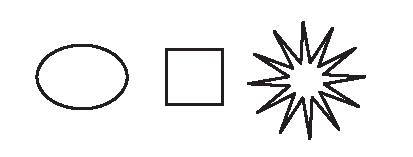
\includegraphics[width=9cm]{poiseuille_shapes.pdf}
\end{center}
\caption{A family of tubes of constant section, but with different shapes.}
\end{figure}

\begin{enumerate}
\item Show the relation:
$$
\mu\left( \frac{\partial^2 u}{\partial y^2} + \frac{\partial^2 u}{\partial z^2} \right) = c.
$$
What is the the meaning of $c$ here?
\item Show that the total viscous force exerted on the wall takes the following expression:
$$
\oiint_{\partial D} \mu \frac{\partial u}{\partial n} \, \mathrm dS.
$$
%    $$
%   \sigma_{xj} (0,n_y,n_z)=\sigma_{xy} n_y + \sigma_{xz} n_z = \mu ( u_{x,y} ) n_y + \mu u_{x,z} n_z = \mu u_{,n}
%    $$
\item On using Green's formulae:
$$
\iiint_V \Psi \nabla^2 \varphi\,\mathrm dV = - \iiint_V \nabla \Psi \cdot \nabla \varphi\,\mathrm dV + \oiint_{\partial V} \Psi \frac{\partial \varphi}{\partial n} \, \mathrm dS,
$$
Answer the question.
\item Show that we could retrieve this result in a blink by conducting a force balance on a fluid portion.
\begin{answer}
The viscous force per unit length is $\pd{p}{x} A$, and does not depend on the tube shape. This result might be surprising at first because we could have expected a more ``dented'' tube, or a tube exposing a higher contact surface, to bear a higher viscous force.
But actually if we consider a fluid portion of length $L$ flowing steadily, we see that the driving force $-\pd{p}{x} A L$ has to be balanced with a resistive force $\tau L$ ($\tau$ being the viscous stress integrated on a section). Hence the result.
\end{answer}

\end{enumerate}
\bibliographystyle{jfm}
\bibliography{biblio_tuto}
\end{document}